% Research theme figure: Complex System Optimization
% (design space -> evolutionary search -> convergence). Same canvas, fonts and palette
% as rom.tex / control.tex; shown in greyscale on the site, colour on hover.
% Hint from: Ayon, Deb, Rahman, Haq, Energy Convers. Manag. X 30 (2026) 101738
% (differential evolution, constrained maximisation), drawn generically.
% Build (from this folder):
%   latex optimization.tex
%   dvisvgm --no-fonts --bbox=papersize -o ../optimization.svg optimization.dvi
\def\pgfsysdriver{pgfsys-dvisvgm.def}
\documentclass[tikz,border=0pt]{standalone}
\usetikzlibrary{arrows.meta}
\renewcommand{\familydefault}{\sfdefault}

% --- palette (shared with rom.tex and control.tex) --------------------------
\definecolor{ink}{HTML}{1A1A1A}
\definecolor{frame}{HTML}{4D4D4D}
\definecolor{steel}{HTML}{245A94}
\definecolor{sky}{HTML}{6E9FD2}
\definecolor{mist}{HTML}{D3E3F3}
\definecolor{amber}{HTML}{C8702A}
\definecolor{sand}{HTML}{F0CFA8}

% objective landscape: global peak (dark) and a weaker local peak
\pgfdeclareradialshading{peakglobal}{\pgfpoint{0bp}{0bp}}{%
  color(0bp)=(steel!95!black); color(10bp)=(steel); color(24bp)=(sky); color(38bp)=(mist); color(50bp)=(mist)}
\pgfdeclareradialshading{peaklocal}{\pgfpoint{0bp}{0bp}}{%
  color(0bp)=(sky!85!steel); color(14bp)=(sky); color(30bp)=(mist); color(50bp)=(mist)}

\begin{document}
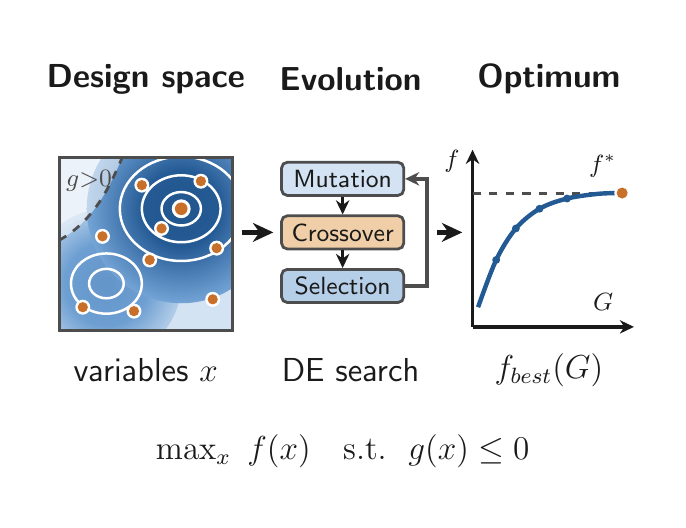
\begin{tikzpicture}[
    line width=1.6pt, >={Stealth[length=2.6mm,width=2.4mm]},
    small arrow/.style={-{Stealth[length=1.8mm,width=1.7mm]}, line width=1.2pt},
    color=ink,
    title/.style={font=\large\bfseries, text=ink},
    lab/.style={font=\large, text=ink},
    stage/.style={draw=frame, line width=1.0pt, rounded corners=2pt, minimum width=1.55cm,
                 minimum height=0.42cm, inner sep=0pt, font=\small, text=ink}]
  % fixed 8 cm x 6 cm canvas
  \path[use as bounding box] (0,0) rectangle (8,6);

  % ================= 1) design space: objective landscape + population =================
  \node[title] at (1.50,5.35) {Design space};
  \begin{scope}
    \clip (0.40,2.15) rectangle (2.60,4.35);
    \fill[mist] (0.40,2.15) rectangle (2.60,4.35);
    \shade[shading=peaklocal]  (1.00,2.75) circle (0.95);
    \shade[shading=peakglobal] (1.95,3.70) circle (1.20);
    \foreach \r in {0.25,0.50,0.78}
      \draw[white, line width=0.9pt] (1.95,3.70) ellipse ({\r} and {0.85*\r});
    \foreach \r in {0.22,0.45}
      \draw[white, line width=0.9pt] (1.00,2.75) ellipse ({\r} and {0.85*\r});
    % infeasible region, g(x) > 0 (upper-left corner)
    \fill[white, opacity=0.55] (0.40,4.35) -- (0.40,3.30) .. controls (0.85,3.55) and (1.05,4.00) .. (1.20,4.35) -- cycle;
    \draw[frame, line width=1.0pt, dashed] (0.40,3.30) .. controls (0.85,3.55) and (1.05,4.00) .. (1.20,4.35);
  \end{scope}
  \node[font=\small, text=frame] at (0.78,4.06) {$g{>}0$};
  \draw[frame, line width=1.0pt] (0.40,2.15) rectangle (2.60,4.35);
  % population of candidate solutions (white ring keeps them visible in greyscale)
  \foreach \p in {(0.70,2.45),(1.35,2.40),(2.35,2.55),(1.55,3.05),(2.40,3.20),(0.95,3.35),(1.70,3.45),(2.20,4.05),(1.45,4.00)} {
    \fill[white] \p circle (0.095);
    \fill[amber] \p circle (0.065);
  }
  % best solution at the global optimum
  \fill[white] (1.95,3.70) circle (0.12);
  \fill[amber] (1.95,3.70) circle (0.08);
  \node[lab] at (1.50,1.65) {variables $x$};

  % ================= 2) evolutionary search (differential evolution) =================
  \node[title] at (4.10,5.35) {Evolution};
  \node[stage, fill=mist] (mu) at (4.00,4.08) {Mutation};
  \node[stage, fill=sand] (cr) at (4.00,3.40) {Crossover};
  \node[stage, fill=sky!50] (se) at (4.00,2.72) {Selection};
  \draw[small arrow] (mu.south) -- (cr.north);
  \draw[small arrow] (cr.south) -- (se.north);
  % next generation loop
  \draw[small arrow, frame] (se.east) -- ++(0.28,0) |- (mu.east);
  \node[lab] at (4.10,1.65) {DE search};

  % ================= 3) convergence to the optimum =================
  \node[title] at (6.62,5.35) {Optimum};
  \draw[small arrow] (5.65,2.20) -- (7.70,2.20);
  \draw[small arrow] (5.65,2.20) -- (5.65,4.45);
  \node[font=\small, anchor=south east] at (7.58,2.26) {$G$};
  \node[font=\small, anchor=east] at (5.63,4.30) {$f$};
  % best objective per generation: fast rise, then plateau at the optimum
  \draw[frame, line width=1.1pt, dashed] (5.65,3.90) -- (7.60,3.90);
  \draw[steel, line width=1.6pt]
    plot[smooth, tension=0.55] coordinates
      {(5.72,2.45) (5.95,3.05) (6.20,3.45) (6.50,3.70) (6.85,3.83) (7.25,3.89) (7.55,3.90)};
  \foreach \p in {(5.95,3.05),(6.20,3.45),(6.50,3.70),(6.85,3.83)}
    \fill[steel] \p circle (0.05);
  \fill[white] (7.55,3.90) circle (0.10);
  \fill[amber] (7.55,3.90) circle (0.07);
  \node[font=\small, anchor=south east] at (7.62,3.95) {$f^{*}$};
  \node[lab] at (6.62,1.65) {$f_{best}(G)$};

  % ================= arrows between panels =================
  \draw[->] (2.72,3.40) -- (3.12,3.40);
  \draw[->] (5.20,3.40) -- (5.52,3.40);

  % ================= problem statement =================
  \node[font=\large, text=ink] at (4.00,0.62)
    {$\max_{x}\ f(x)\quad \mathrm{s.t.}\ \ g(x)\le 0$};
\end{tikzpicture}
\end{document}
